\textbf{COLUNI 2021 -- Questão 34}\par\medskip Observe a imagem e leia o texto a seguir.

% COLUNI-AUTO-FIGURES-BEGIN
\begin{figure}[htbp]
\centering
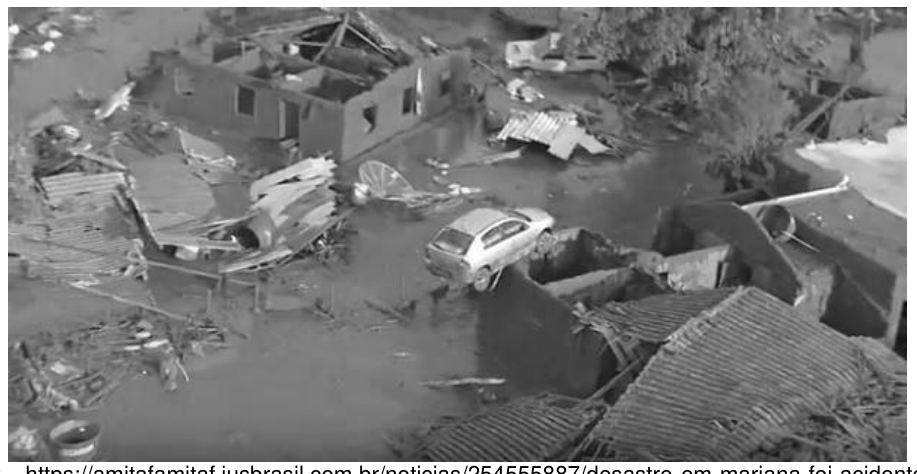
\includegraphics[width=0.95\linewidth]{static/simulados/coluni/figuras/2021/questao-34/figura-1.png}
\end{figure}
% COLUNI-AUTO-FIGURES-END

Disponível em: https://amitafamitaf.jusbrasil.com.br/noticias/254555887/desastre-em-mariana-foi-acidente-ou-crime-e-precipitado-avaliar-diz-ministro. Acesso em: 01 dez. 2020.

\par

\textbf{Tragédia de Mariana, 5 anos: sem julgamento ou recuperação ambiental [...].}

\par

Esperança, preparação para o inesperado, injustiça, tristeza e revolta. Nesta quinta-feira (05/11/2020), o rompimento da barragem de Fundão, em Mariana (MG), completa cinco anos […]. A barragem da Samarco, cujas donas são a Vale e BHP Billiton, rompeu-se na tarde do dia 5 de novembro de 2015, provocando 19 mortes. Além de destruir casas, o mar de lama devastou o Rio Doce e atingiu o oceano no Espírito Santo. Nestes mais de 1,8 mil dias, os responsáveis pela tragédia não foram julgados. Em 2019, o crime de homicídio foi retirado do processo. As mortes provocadas pelo rompimento da barragem foram consideradas pela Justiça como consequência da inundação causada pelo rompimento. Durante este período, as comunidades destruídas não foram reconstruídas e ainda faltam respostas para a recuperação do meio ambiente. [...]

\par

Disponível em: https://g1.globo.com/mg/minas-gerais/noticia/2020/11/05/tragedia-de-mariana-5-anos-sem-julgamentoou-recuperacao-ambiental-5-vidas-contam-os-impactos-no-periodo.ghtml. Acesso em: 01 dez. 2020. (Adaptado).

\par

Sobre a tragédia de Mariana, é CORRETO afirmar que:

\begin{enumerate}
\item ocorreu na região sul de Minas Gerais, banhada pela bacia do Rio Doce, que é fortemente influenciada
      pelo clima subtropical em função da altitude de seu relevo.
\item ao verem soterrados os distritos Paracatu de Baixo e Bento Rodrigues, as pessoas que ali viviam
      perderam também a referência de lugar.
\item a tragédia de Mariana impactou negativamente apenas os pequenos agricultores e os proprietários rurais
      que tinham suas terras ao longo do Rio Doce no estado de Minas Gerais.
\item o impacto ambiental dessa tragédia não provocou grandes danos marinhos na foz do Rio Doce, localizada no
      estado do Espírito Santo, porque as correntes marinhas levaram e depositaram os rejeitos em alto-mar.
\end{enumerate}
